\documentclass[11pt,a4paper]{article}
\usepackage{float}
\usepackage{wrapfig}
\usepackage{amsmath}
\usepackage{graphicx}
\usepackage{listings}
\usepackage{enumitem}
\usepackage[dvipsnames]{xcolor}
\usepackage[linktoc=none]{hyperref}
\usepackage[justification=centering]{caption}
\usepackage[a4paper, portrait, margin=1.2in]{geometry}
\usepackage[framed, autolinebreaks, useliterate]{mcode}
\hypersetup{
    colorlinks=true,
    linkcolor=blue,
    filecolor=magenta,      
    urlcolor=blue,
}
\lstset{aboveskip=\medskipamount}
\begin{document}
\begin{center}
    \Large\textbf{Stock Market time series analysis using OpenStack, Gnocchi and Grafana}\\
    \vspace{0.2cm}
    \large{Cloud Computing final project - Prof. Carlo Vallati}\\
    \vspace{1.0cm}
    \large\textit{Leonardo Turchetti}\\
    \large\textit{Lorenzo Tonelli}\\
    \large\textit{Ludovica Cocchella}\\
    \large\textit{Rambod Rahmani}\\
    \vspace{0.2cm}
    \normalsize{Msc. in Artificial Intelligence and Data Engineering}\\
    \vspace{1.0cm}
    \today
\end{center}
\vspace{1cm}
\tableofcontents
\vspace{1cm}
\section{Introduction}
The project focused on deploying Gnocchi - an open-source time series database - and Grafana - an open source analytics and monitoring solution - on the preexisting OpenStack installation. After deployment, some preliminary tests were carried out in order to make sure everything was running smoothly. Finally, Gnocchi metrics were created and populated using stock market data. Grafana was then used to visualize the data and extract useful statistics.\\
\\
In what follows, the deployment procedures and the ad-hoc required configurations are detailed. Just for reference, the preexisting OpenStack installation consists of:
\begin{lstlisting}[numbers=left]
172.16.3.218    Juju Controller
172.16.3.238    Compute Node 0/OpenStack Controller
172.16.3.177    Compute Node 1
172.16.3.174    Compute Node 2
172.16.3.227    Compute Node 3
\end{lstlisting}
The entire codebase is available at \url{https://github.com/lorytony/CloudComputing}.
\section{Gnocchi Deployment}
Gnocchi is an open-source time series database. The problem that Gnocchi solves is the storage and indexing of time series data and resources at a large scale. Gnocchi takes a unique approach to time series storage: rather than storing raw data points, it aggregates them before storing them. This built-in feature is different from most other time series databases, which usually support this mechanism as an option and compute aggregation (average, minimum, etc.) at query time.\\
\\
The Gnocchi database was deployed\footnote{\url{https://jaas.ai/gnocchi/37}} to compute node 0 in a container using Juju
\begin{lstlisting}[]
$ juju deploy --to lxd:0 cs:gnocchi
$ juju deploy --to lxd:0 cs:memcached
$ juju add-relation gnocchi mysql
$ juju add-relation gnocchi memcached
$ juju add-relation gnocchi keystone
$ juju add-relation gnocchi ceph-mon
\end{lstlisting}
The choice was made to deploy Gnocchi inside a container. As a result, initially, Gnocchi was accessible only from the OpenStack controller node. For ease of debugging, port forwarding was applied on the OpenStack controller node in order to make Gnocchi visible from outside.
\begin{lstlisting}[]
$ iptables -t nat -A PREROUTING -i eth0 -p tcp -m tcp --dport 5000 -j DNAT --to-destination 252.3.238.205:5000
$ iptables -t nat -A POSTROUTING -d 252.3.238.205/32 -o eth0 -j MASQUERADE

$ iptables -t nat -A PREROUTING -i eth0 -p tcp -m tcp --dport 8041 -j DNAT --to-destination 252.3.238.176:8041
$ iptables -t nat -A POSTROUTING -d 252.3.238.176/32 -o eth0 -j MASQUERADE
\end{lstlisting}
From within the OpenStack network and from outside, Gnocchi can now be accessed using the OpenStack controller IP address:
\begin{lstlisting}[]
$ source admin-openrc.sh
$ openstack token issue
$ gnocchi --endpoint http://172.16.3.238:8041 metric list
\end{lstlisting}
Right after deployment, some preliminary tests - creating a metric, pushing and reading measurements - were performed using Gnocchi REST API to check if the deployment was successful.
\subsection{Metrics}
Gnocchi is based on the concept of metrics which contain measurements: as we intend to store stock market data, a new metric was created for each of the stocks we intend to monitor. The top $15$ stocks of the NASDAQ Stock Exchange were selected.\\
\\
The official Gnocchi Python client was used to create the required metrics:
\begin{lstlisting}[]
$ gnocchi metric create --archive-policy-name high "GOOG"
$ gnocchi metric create --archive-policy-name high "ADSK"
$ gnocchi metric create --archive-policy-name high "FOX"
$ gnocchi metric create --archive-policy-name high "EBAY"
$ gnocchi metric create --archive-policy-name high "AMD"
...
\end{lstlisting}
The default \texttt{archive-policy} used is \texttt{high}. By default, $4$ archive policies are available. The name both describes the storage space and CPU usage needs.
\begin{itemize}[noitemsep]
    \item low
    \begin{itemize}
        \item 5 minutes granularity over 30 days;
    \end{itemize}
    \item medium
    \begin{itemize}
        \item 1 minute granularity over 7 days;
        \item 1 hour granularity over 365 days;
    \end{itemize}
    \item high
    \begin{itemize}
        \item 1 second granularity over 1 hour;
        \item 1 minute granularity over 1 week;
        \item 1 hour granularity over 1 year.
    \end{itemize}
\end{itemize}
The archive policies define how the metrics are aggregated and how long they are stored. Each archive policy definition is expressed as the number of points over a timespan. Each archive policy also defines which aggregation methods will be used. The default is set to \texttt{default\_aggregation\_methods} which is by default set to \texttt{mean}, \texttt{min}, \texttt{max}, \texttt{sum}, \texttt{std}, \texttt{count}.\\
\\
Both the archive policy and the granularity entirely depend on your use case. For our intended usage, the default \texttt{archive-policy} \texttt{high} and the default aggregations methods were considered more than enough. Be aware that the more definitions you set in an archive policy, the more CPU it will consume.
\section{Grafana Deployment}
Grafana is a multi-platform open source analytics and interactive visualization web application. It provides charts, graphs, and alerts for the web when connected to supported data sources. It is expandable through a plug-in system. End users can create complex monitoring dashboards using interactive query builders.\\
\\
Grafana was deployed\footnote{\url{https://jaas.ai/grafana/40}} to compute node 0 using Juju
\begin{lstlisting}[]
$ juju deploy cs:grafana
\end{lstlisting}
The choice was made not to deploy Grafana inside a container in order to be able to easily access its web interface and avoid further configurations related to port forwarding.
\subsection{Gnocchi Datasource}
The Gnocchi datasource was installed via grafana.net\footnote{\url{https://grafana.com/grafana/plugins/gnocchixyz-gnocchi-datasource}}:
\begin{lstlisting}[]
$ grafana-cli plugins install gnocchixyz-gnocchi-datasource
$ systemctl restart grafana-server
\end{lstlisting}
Finally, a new Gnocchi data source was added using the Grafana web interface:
\begin{figure}[H]
    \centering
    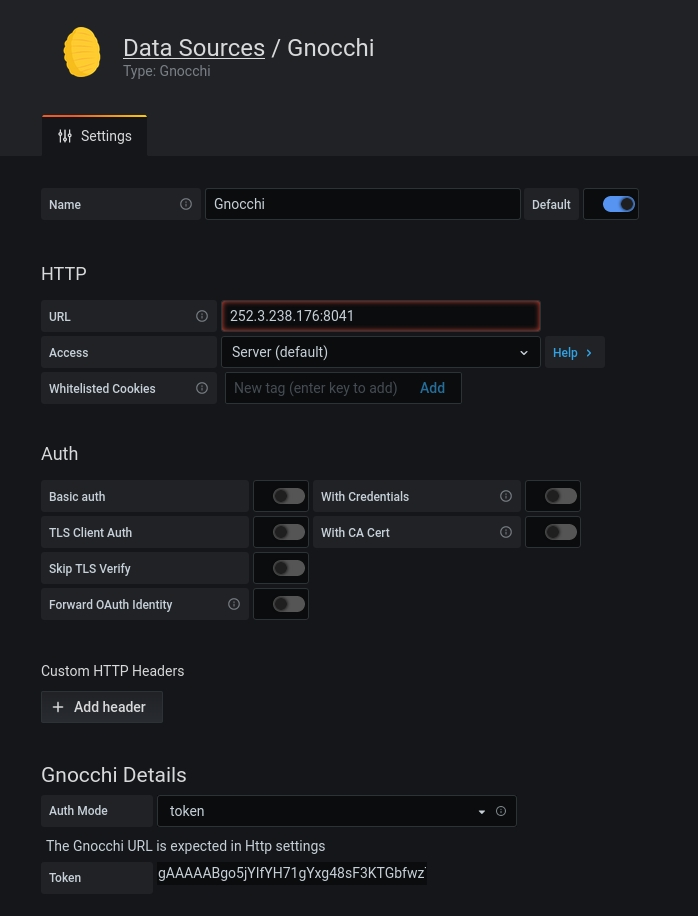
\includegraphics[scale=0.65]{imgs/grafana-gnocchi-datasource.jpg}
\end{figure}
\noindent
As it can be seen in the previous picture, Grafana needs a Keystone token as part of the Gnocchi data source configuration. In order to avoid having issues related to expiring authentication tokens, the default Keystone \texttt{token-expiration} ($3600$ $s$) parameter was changed to one month ($2628000$ $s$):
\begin{lstlisting}[]
root@namenode:# juju config keystone token-expiration=2628000
root@namenode:# juju config keystone
...
  token-expiration:
    default: 3600
    description: Amount of time (in seconds) a token should remain valid.
    source: user
    type: int
    value: 2.628e+06
...
\end{lstlisting}
\begin{lstlisting}[]
root@namenode:# openstack token issue
+------------+-------------------------------------------------------------+
| Field      | Value                                                       |
+------------+-------------------------------------------------------------+
| expires    | 2021-06-23T01:51:22+0000                                    |
| id         | gAAAAABgqnn6SkcwKpsGhVa79RqhNr4jwf8je4r9X3LwgLEApA_98m4KqXp |
| project_id | 3d10367c76574f36a007ce9c90761f50                            |
| user_id    | afd3ffcbb426446296ab30c898581355                            |
+------------+-------------------------------------------------------------+
\end{lstlisting}
\section{Fetching Stock Market Data}
In order to fetch stock market data a Python3 script was written initially using the Yahoo! Finance\footnote{\url{https://finance.yahoo.com/}} API. However, being a freely available service, it was not reliable enough in order to be able provide real time data.\\
\\
Therefore, a new implementation was developed using IEX Cloud\footnote{\url{https://iexcloud.io}} with an educational license. Thanks to this new provider, we were able to fetch real time stock market data as well as leverage upon the \texttt{sandbox} functionality they provide in order to obtain randomized realistic test data when the stock market is closed (regular trading hours for the U.S. stock market, including the New York Stock Exchange (NYSE) and the Nasdaq Stock Market (Nasdaq), are 9:30 a.m. to 4 p.m. Eastern time on weekdays).
\begin{lstlisting}[language=python,caption={fetch\_stock\_prices.py},numbers=left]
#!/usr/bin/env python

import pyEX
import json
import urllib.request
from datetime import datetime

# pyEX engine
c = pyEX.Client("pk_e58014e8a6bd415d8af6e459f2353eb5")

# keystone token
keystone_token = "gAAAAABgqo4EBJerAKtAUGHMUyE93A7Vnoy3XUXZ7lLOGLXki_qXc..."

# stock tickers to be retrieved
tickers = ["AMZN", "GOOG", "BKNG", "CHTR", "NVDA", "TSLA", "NFLX", ...];
tickers_metrics = ["a34a5ffb-a616-4583-99df-73885cbac719", \ ...]

try:
    while True:
        for i in range(len(tickers)):
            timestamp = datetime.utcnow().strftime("%Y-%m-%dT%H:%M:%S")
            price = c.price(tickers[i])
            print(timestamp + " | " + tickers[i] + " - " + str(price))

            if (price > 0.0):
                # push data to gnocchi
                conditionsSetURL = "http://252.3.238.176:8041/v1/metric/" ...
                newConditions = [{"timestamp": timestamp, "value": ...
                params = json.dumps(newConditions).encode('utf8')
                req = urllib.request.Request(conditionsSetURL, data= ...
                urllib.request.urlopen(req)
except Exception:
    print("Exception fetching stock market data. Ignoring.")
    pass
\end{lstlisting}
The full commented source code of this listing can be found in the GitHub repository under \texttt{vallati/python/fetch\_stock\_prices.py}. For each of the stock market tickers defined, also the corresponding Gnocchi metric ID is defined. For each stock, the market price of the current trading session is fetched and pushed to Gnocchi. All timestamps are converted to UTC timezone, as expected by Gnocchi.
\subsection{Docker Container}
A custom Docker container was deployed on the OpenStack controller VM in order to keep the Python script going:
\begin{lstlisting}[numbers=left, caption={Dockerfile}]
# start from an official ubuntu image
FROM ubuntu

# specify the command to be run inside the container at installation
RUN apt-get update && apt-get install -y python3 python3-pip
RUN python3 -m pip install --no-cache-dir --upgrade pip && \
    python3 -m pip install --no-cache-dir gnocchiclient pyEX pandas

# add some file to the image from the host
ADD ./fetch_stock_prices.py /root/

# at startup, run the following command
CMD ["/usr/bin/python3", "/root/fetch_stock_prices.py"]
\end{lstlisting}
\begin{lstlisting}[]
root@controller:# docker build -t fetch-stock-prices .

root@controller:# docker run -d fetch-stock-prices
3a38875721a9fed598b69848ce7a9da0166a1b92868720811f43b2b7ad0e4716

root@controller:# docker ps -a
CONTAINER ID  IMAGE               COMMAND                  CREATED
3a38875721a9  fetch-stock-prices  "/usr/bin/python3 /r."   6 seconds
\end{lstlisting}
\section{Grafana Dashboard}
A dashboard is a set of one or more panels organized and arranged into one or more rows. Grafana ships with a variety of Panels. Grafana makes it easy to construct the right queries, and customize the display properties so that you can create the perfect dashboard for your need. Each panel can interact with data from any configured Grafana Data Source. A dashboard in Grafana is represented by a JSON object, which stores metadata of its dashboard. Dashboard metadata includes dashboard properties, metadata from panels, template variables, panel queries, etc.
\subsection{Stock Market Dashboard}
A custom dashboard was developed using Grafana web interface.
\begin{figure}[H]
    \centering
    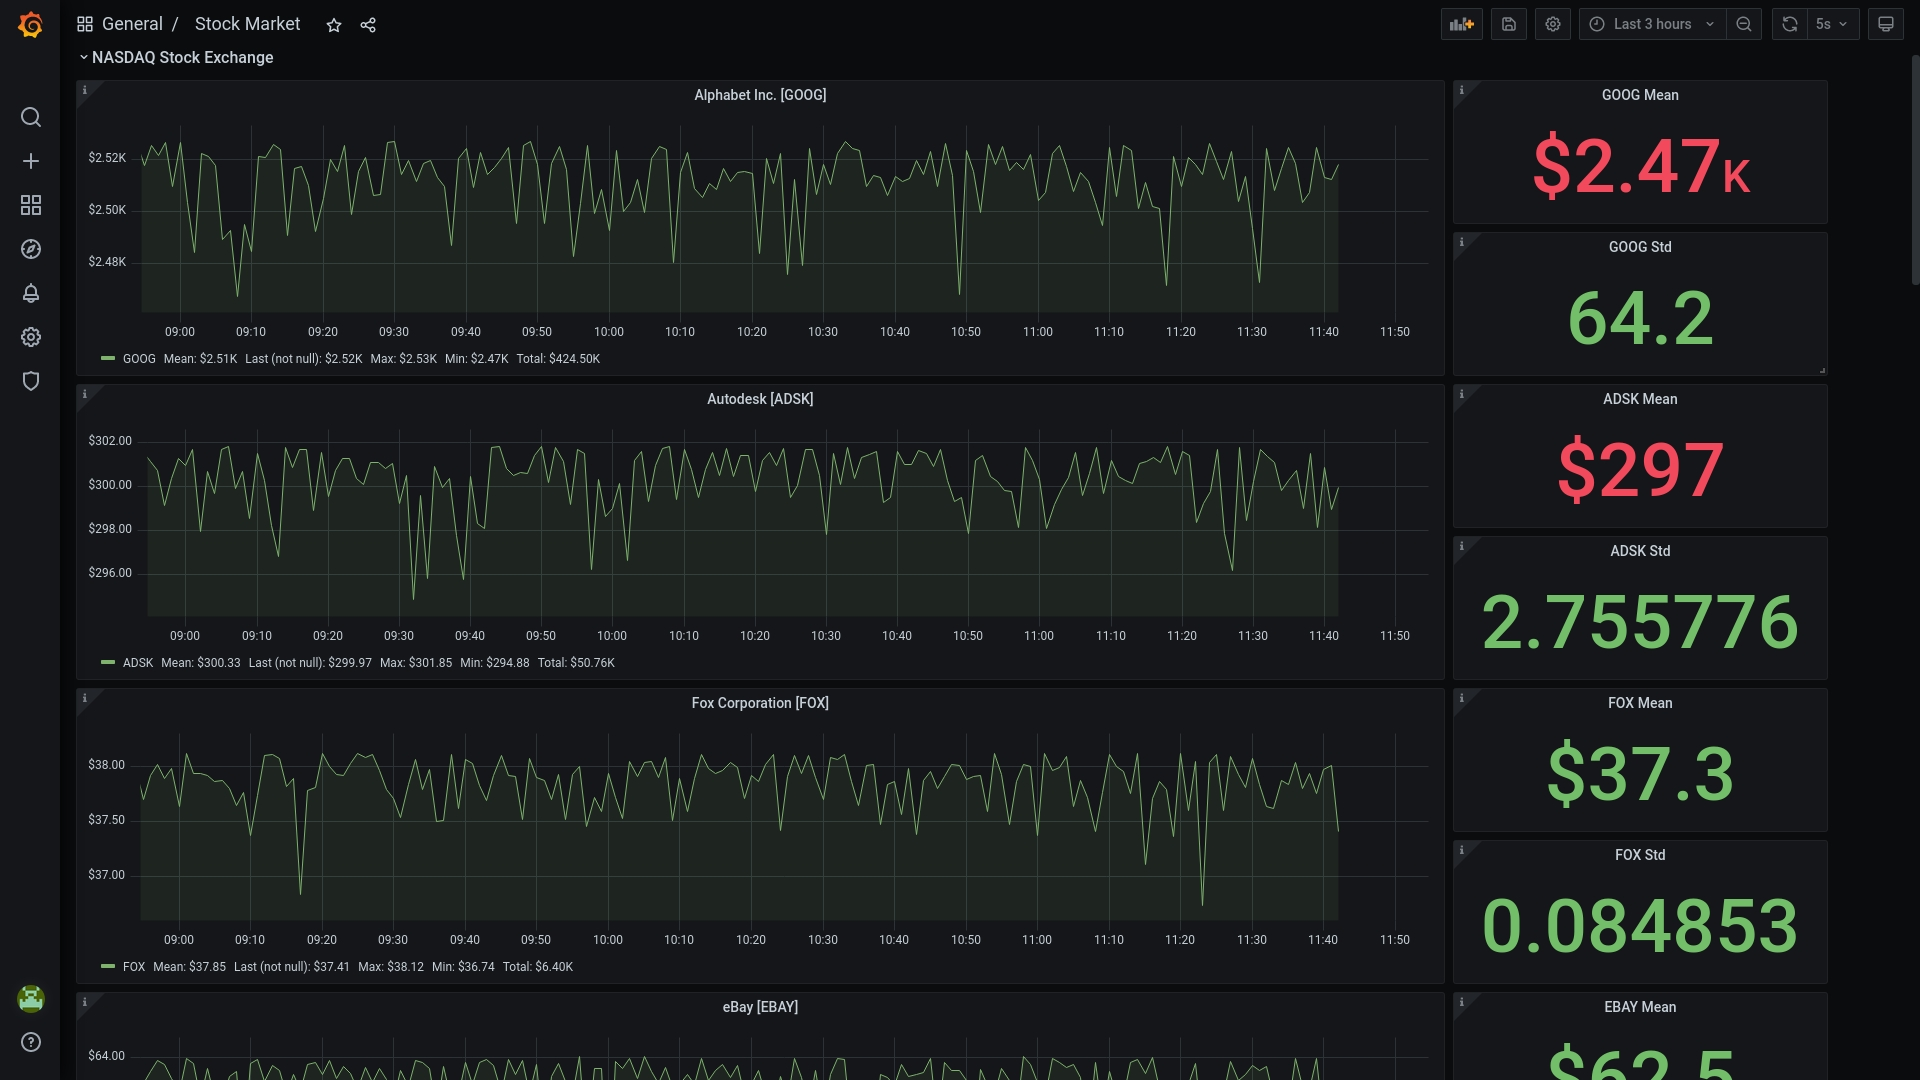
\includegraphics[scale=0.245]{imgs/grafana-dashboard.jpg}
\end{figure}
\noindent
For each stock, the following information is displayed:
\begin{itemize}
    \item stock price time series plot;
    \item stock average price;
    \item stock price standard deviation: this is a statistical measure of market volatility, measuring how widely prices are dispersed from the average price.
\end{itemize}
\section{Future work}
The current deployment can be improved pushing it to the extreme as follows:
\begin{itemize}
    \item create a new Gnocchi archive policy with a granularity of $1$ second over a timespan of $1$ year;
    \item create custom Gnocchi aggregation methods;
    \item for each stock store the open, high, low, close and volume values;
    \item run a dedicated docker container for each of the stocks we want to monitor in order to be able to fetch data as fast as possible;
    \item for each stock, compute and display the candlestick chart and useful statistics using a Grafana dashboard.
\end{itemize}
\begin{figure}[H]
    \centering
    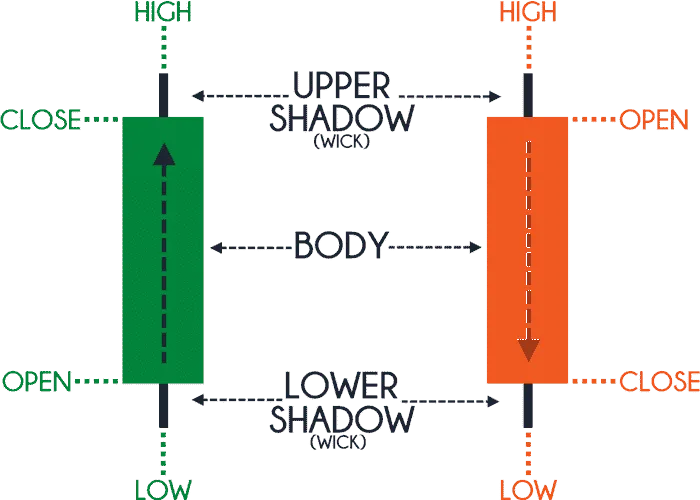
\includegraphics[scale=0.41]{imgs/ohlc-explained.png}
    \caption{Open-High-Low-Close Chart Explained}
\end{figure}
\begin{figure}[H]
    \centering
    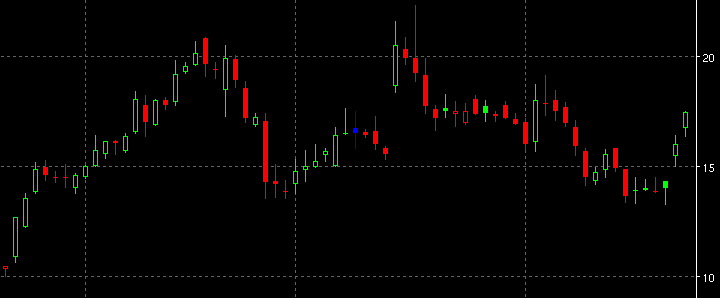
\includegraphics[scale=0.585]{imgs/candlestickchart.png}
    \caption{Candlestick Chart}
\end{figure}
\end{document}